\documentclass[12pt]{beamer}
\usepackage{../Estilos/BeamerFC}
\usepackage{../Estilos/ColoresLatex}
\usepackage{courier}
\usepackage{listingsutf8}
\usepackage{listings}
\usepackage{xcolor}
\usepackage{textcomp}
\usepackage{color}
\definecolor{deepblue}{rgb}{0,0,0.5}
\definecolor{brown}{rgb}{0.59, 0.29, 0.0}
\definecolor{OliveGreen}{rgb}{0,0.25,0}
% \usepackage{minted}

\DeclareCaptionFont{white}{\color{white}}
\DeclareCaptionFormat{listing}{\colorbox{gray}{\parbox{0.98\textwidth}{#1#2#3}}}
\captionsetup[lstlisting]{format=listing,labelfont=white,textfont=white}
\renewcommand{\lstlistingname}{Código}


\definecolor{Code}{rgb}{0,0,0}
\definecolor{Keywords}{rgb}{255,0,0}
\definecolor{Strings}{rgb}{255,0,255}
\definecolor{Comments}{rgb}{0,0,255}
\definecolor{Numbers}{rgb}{255,128,0}

\makeatletter

\newif\iffirstchar\firstchartrue
\newif\ifstartedbyadigit
\newif\ifprecededbyequalsign

\newcommand\processletter
{%
  \ifnum\lst@mode=\lst@Pmode%
    \iffirstchar%
        \global\startedbyadigitfalse%
      \fi
      \global\firstcharfalse%
    \fi
}

\newcommand\processdigit
{%
  \ifnum\lst@mode=\lst@Pmode%
      \iffirstchar%
        \global\startedbyadigittrue%
      \fi
      \global\firstcharfalse%
  \fi
}

\lst@AddToHook{OutputOther}%
{%
  \lst@IfLastOtherOneOf{=}
    {\global\precededbyequalsigntrue}
    {}%
}

\lst@AddToHook{Output}%
{%
  \ifprecededbyequalsign%
      \ifstartedbyadigit%
        \def\lst@thestyle{\color{orange}}%
      \fi
    \fi
  \global\firstchartrue%
  \global\startedbyadigitfalse%
  \global\precededbyequalsignfalse%
}

\lstset{ 
language=Python,                % choose the language of the code
basicstyle=\footnotesize\ttfamily,       % the size of the fonts that are used for the code
numbers=left,                   % where to put the line-numbers
numberstyle=\scriptsize,      % the size of the fonts that are used for the line-numbers
stepnumber=1,                   % the step between two line-numbers. If it is 1 each line will be numbered
numbersep=5pt,                  % how far the line-numbers are from the code
backgroundcolor=\color{white},  % choose the background color. You must add \usepackage{color}
showspaces=false,               % show spaces adding particular underscores
showstringspaces=false,         % underline spaces within strings
showtabs=false,                 % show tabs within strings adding particular underscores
frame=single,   		% adds a frame around the code
tabsize=2,  		% sets default tabsize to 2 spaces
captionpos=t,   		% sets the caption-position to bottom
breaklines=true,    	% sets automatic line breaking
breakatwhitespace=false,    % sets if automatic breaks should only happen at whitespace
escapeinside={| |},  % if you want to add a comment within your code
stringstyle =\color{OliveGreen},
otherkeywords={as, np.array, np.concatenate, np.linspace, linspace, interpolate.interp1d, kind, plt.plot, .copy, np.arange, np.cos, np.pi, lw, ls, label, splrep, splev, plt.legend, loc, plt.title, plt.ylim, plt.show, sign, math.ceil, math.log, np.sqrt, np.exp, np.zeros, plt.xlabel, plt.ylabel, plt.xlim, np.identity, random, np.dot, np.outer, np.diagonal },             % Add keywords here
keywordstyle = \color{blue},
commentstyle = \color{darkcerulean},
identifierstyle = \color{black},
literate=%
         {á}{{\'a}}1
         {é}{{\'e}}1
         {í}{{\'i}}1
         {ó}{{\'o}}1
         {ú}{{\'u}}1
%
%keywordstyle=\ttb\color{deepblue}
%fancyvrb = true,
}

\lstdefinestyle{FormattedNumber}{%
    literate={0}{{\textcolor{red}{0}}}{1}%
             {1}{{\textcolor{red}{1}}}{1}%
             {2}{{\textcolor{red}{2}}}{1}%
             {3}{{\textcolor{red}{3}}}{1}%
             {4}{{\textcolor{red}{4}}}{1}%
             {5}{{\textcolor{red}{5}}}{1}%
             {6}{{\textcolor{red}{6}}}{1}%
             {7}{{\textcolor{red}{7}}}{1}%
             {8}{{\textcolor{red}{8}}}{1}%
             {9}{{\textcolor{red}{9}}}{1}%
             {.0}{{\textcolor{red}{.0}}}{2}% Following is to ensure that only periods
             {.1}{{\textcolor{red}{.1}}}{2}% followed by a digit are changed.
             {.2}{{\textcolor{red}{.2}}}{2}%
             {.3}{{\textcolor{red}{.3}}}{2}%
             {.4}{{\textcolor{red}{.4}}}{2}%
             {.5}{{\textcolor{red}{.5}}}{2}%
             {.6}{{\textcolor{red}{.6}}}{2}%
             {.7}{{\textcolor{red}{.7}}}{2}%
             {.8}{{\textcolor{red}{.8}}}{2}%
             {.9}{{\textcolor{red}{.9}}}{2}%
             {\ }{{ }}{1}% handle the space
         ,%
          %mathescape=true
          escapeinside={__}
          }



\usetheme{Copenhagen}
\usecolortheme{wolverine}
%\useoutertheme{default}
\setbeamercovered{invisible}
% or whatever (possibly just delete it)
\setbeamertemplate{section in toc}[sections numbered]
\setbeamertemplate{subsection in toc}[subsections numbered]
\setbeamertemplate{subsection in toc}{\leavevmode\leftskip=3.2em\rlap{\hskip-2em\inserttocsectionnumber.\inserttocsubsectionnumber}\inserttocsubsection\par}
% \setbeamercolor{section in toc}{fg=blue}
% \setbeamercolor{subsection in toc}{fg=blue}
% \setbeamercolor{frametitle}{fg=blue}
\setbeamertemplate{caption}[numbered]

\setbeamertemplate{footline}
\beamertemplatenavigationsymbolsempty
\setbeamertemplate{headline}{}


\makeatletter
% \setbeamercolor{section in foot}{bg=gray!30, fg=black!90!orange}
% \setbeamercolor{subsection in foot}{bg=blue!30}
% \setbeamercolor{date in foot}{bg=black}
\setbeamertemplate{footline}
{
  \leavevmode%
  \hbox{%
  \begin{beamercolorbox}[wd=.333333\paperwidth,ht=2.25ex,dp=1ex,center]{section in foot}%
    \usebeamerfont{section in foot} \insertsection
  \end{beamercolorbox}%
  \begin{beamercolorbox}[wd=.333333\paperwidth,ht=2.25ex,dp=1ex,center]{subsection in foot}%
    \usebeamerfont{subsection in foot}  \insertsubsection
  \end{beamercolorbox}%
  \begin{beamercolorbox}[wd=.333333\paperwidth,ht=2.25ex,dp=1ex,right]{date in head/foot}%
    \usebeamerfont{date in head/foot} \insertshortdate{} \hspace*{2em}
    \insertframenumber{} / \inserttotalframenumber \hspace*{2ex} 
  \end{beamercolorbox}}%
  \vskip0pt%
}
\makeatother

\makeatletter
\patchcmd{\beamer@sectionintoc}{\vskip1.5em}{\vskip0.8em}{}{}
\makeatother

% %\newlength{\depthofsumsign}
% \setlength{\depthofsumsign}{\depthof{$\sum$}}
% \newcommand{\nsum}[1][1.4]{% only for \displaystyle
%     \mathop{%
%         \raisebox
%             {-#1\depthofsumsign+1\depthofsumsign}
%             {\scalebox
%                 {#1}
%                 {$\displaystyle\sum$}%
%             }
%     }
% }
% \def\scaleint#1{\vcenter{\hbox{\scaleto[3ex]{\displaystyle\int}{#1}}}}
% \def\scaleoint#1{\vcenter{\hbox{\scaleto[3ex]{\displaystyle\oint}{#1}}}}
% \def\bs{\mkern-12mu}

\usefonttheme{serif}

\title{\large{RK4, Estabilidad y Rigidez de las EDO}}
\subtitle{Tema 3 - Ecuaciones Diferenciales Ordinarias}
\author{M. en C. Gustavo Contreras Mayén}
\date{}

\begin{document}
\maketitle

\section*{Contenido}
\frame{\tableofcontents[currentsection, hideallsubsections]}

\section{Runge-Kutta de cuarto orden}
\frame[allowframebreaks]{\tableofcontents[currentsection, hideothersubsections]}
\subsection{El método}

\begin{frame}
\frametitle{Obteniendo el método}
El \textcolor{cadmiumgreen}{método de Runge-Kutta de cuarto orden} (RK4) se obtiene de la serie de Taylor de la misma manera que el método de segundo orden.
\\
\bigskip
\pause
Debido a que la derivación es bastante larga y no muy instructiva, la omitiremos.
\end{frame}
\begin{frame}
\frametitle{Operaciones para el RK4}
La forma final de la fórmula de integración nuevamente depende de la elección de los parámetros; \pause es decir, no existe una fórmula única para el RK4.
\end{frame}
\begin{frame}
\frametitle{Versión para el RK4}
La versión más popular, que se conoce simplemente como \textcolor{cornellred}{método de Runge-Kutta}, implica la siguiente secuencia de operaciones:
\end{frame}
\begin{frame}
\frametitle{Versión para el RK4}
\begin{align}
\begin{aligned}
\mathbf{K_{0}} &= h \, \mathbf{F} (x, \mathbf{y}) \\
\mathbf{K_{1}} &= h \, \mathbf{F} \bigg[x + \dfrac{h}{2}, \mathbf{y} + \dfrac{\mathbf{K}_{0}}{2} \bigg] \\
\mathbf{K_{2}} &= h \, \mathbf{F} \bigg[x + \dfrac{h}{2}, \mathbf{y} + \dfrac{\mathbf{K}_{1}}{2} \bigg] \\
\mathbf{K_{3}} &= h \, \mathbf{F} \big[x + h, \mathbf{y} + \mathbf{K}_{2} \big] \\
\mathbf{y} (x + h) &= \mathbf{y} (x) + \dfrac{1}{6} \bigg[ \mathbf{K}_{0} + 2 \, \mathbf{K_{1}} + 2 \, \mathbf{K_{2}} + \mathbf{K_{3}} \bigg]
\end{aligned}
\label{eq:ecuacion_07_10}
\end{align}
\end{frame}
\begin{frame}
\frametitle{Desventaja del RK4}
El principal inconveniente de este método es que no se presta a una estimación del error de truncamiento.
\\
\bigskip
\pause
Por lo tanto, debemos adivinar el tamaño del paso de integración $h$ o determinarlo por prueba y error.
\end{frame}
\begin{frame}
\frametitle{Otro tipo de métodos}
Por el contrario, los llamados \textcolor{darkcerulean}{métodos adaptativos} pueden evaluar el error de truncamiento en cada paso de integración y ajustar el valor de $h$ en consecuencia (pero a un mayor costo de cálculo).
\end{frame}
\begin{frame}
\frametitle{Propuesta de código}
La función \funcionazul{integraorden4} implementa el método RK4.
\\
\bigskip
\pause
El usuario debe de proporcionar la función \texttt{F (x, y)} que define el sistema de EDO1.
\end{frame}
\begin{frame}[allowframebreaks, fragile]
\frametitle{Código}
\begin{lstlisting}[caption=Código para el método RK4]
def integraorden4(F, x, y, xAlto, h):

    def run_kut4(F, x, y, h):
        K0 = h * F(x, y)
        K1 = h * F(x + h/2., y + K0/2.)
        K2 = h * F(x + h/2., y + K1/2.)
        K3 = h * F(x + h, y + K2)
        
        return (K0 + 2. * K1 + 2. * K2 + K3) / 6.
    
    X = []
    Y = []
    X.append(x)
    Y.append(y)
    
    while x < xAlto:
        h = min(h, xAlto - x)
        y += run_kut4(F, x, y, h)
        x += h
        X.append(x)
        Y.append(y)
    
    return np.array(X), np.array(Y)
\end{lstlisting}
\end{frame}

\subsection{Ejercicio 1 con RK4}

\begin{frame}
\frametitle{Ejercicio a resolver}
Resuelve el siguiente problema de valores iniciales:
\pause
\begin{align*}
\sderivada{y} = -0.1 \, \pderivada{y} - x \hspace{1cm} y (0) = 0 \hspace{0.7cm} \pderivada{y} (0) = 1
\end{align*}
con RK4, de $x = 0$ a $x = 2$ en incrementos de $h = 0.2$. \pause Grafica la solución numérica $y$ y compara con la solución analítica:
\pause
\begin{align*}
y = 100 \, x - 5 \, x^{2} + 990 \, \big( e^{-0.1 x} - 1 \big)
\end{align*}
\end{frame}
\begin{frame}
\frametitle{Ejercicio resuelto con RK2}
Este ejercicio se trabajó con RK2:
\pause
\begin{align*}
\mathbf{F} (x, \mathbf{y}) = 
\begin{bmatrix}
\pderivada{y}_{0} \\
\pderivada{y}_{1}
\end{bmatrix} =
\begin{bmatrix}
y_{1} \\
-0.1 \, y_{1} - x
\end{bmatrix}
\hspace{1.5cm}
\mathbf{y} (0) = 
\begin{bmatrix}
0 \\
1
\end{bmatrix}
\end{align*}
\end{frame}
\begin{frame}[allowframebreaks, fragile]
\frametitle{Código para el ejercicio RK4}
\begin{lstlisting}[caption=Código para resolver el ejercicio con el método RK4]
from metodosDirectos import integraorden4
import numpy as np

def f(x, y):
	f = np.zeros(2)
	f[0] = y[1]
	f[1] = -0.1 * y[1] - x
	return f

x = 0.0
xAlto = 2.0
y = np.array([0., 1.])
h = 0.2

X, Y = integraorden4(f, x, y, xAlto, h)
s_Exacta = 100. * X - 5. * X**2 + 990. *(np.exp(-0.1 * X) - 1.)
\end{lstlisting}
\end{frame}
\begin{frame}
\frametitle{Gráfica de la solución}
\begin{figure}
	\centering
	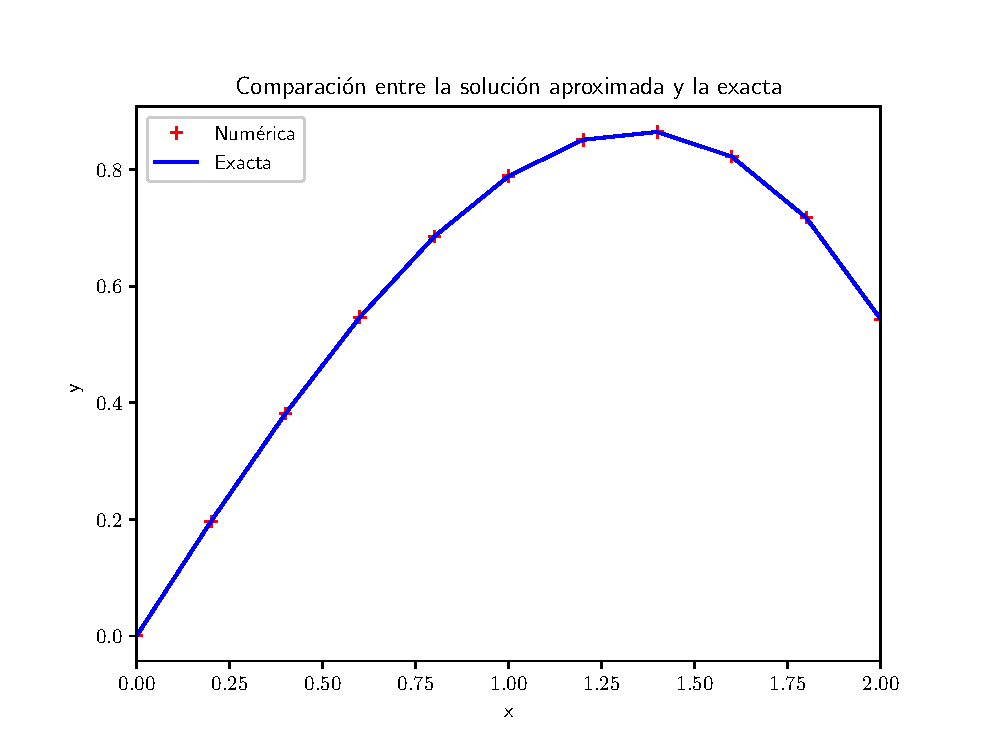
\includegraphics[scale=0.55]{Imagenes/plot_rk4_ejercicio_01.eps}
\end{figure}
\end{frame}

\subsection{Ejercicio 2 RK4}

\begin{frame}
\frametitle{Enunciado del Ejercicio 2}
Con el método RK4 resuelve el siguiente problema:
\pause
\begin{align*}
\pderivada{y} = 3 \, y - 4 \, e^{-x} \hspace{1cm} y (0) = 1
\end{align*}
de $x = 0$ a $10$ en pasos de $h = 0.1$. \pause Compara el resultado con la solución analítica:
\pause
\begin{align*}
y = e^{-x}
\end{align*}
\end{frame}
\begin{frame}
\frametitle{Notación}
Usamos la notación:
\pause
\begin{align*}
\mathbf{F} (x, \mathbf{y}) = 
\begin{bmatrix}
\pderivada{y}_{0} 
\end{bmatrix} =
\begin{bmatrix}
3 * y[0] - 4 * exp(-x)
\end{bmatrix}
\hspace{1cm}
\mathbf{y} (0) = 
\begin{bmatrix}
1
\end{bmatrix}
\end{align*}
\end{frame}
\begin{frame}
\frametitle{Gráfica de la solución exacta}
\begin{figure}
	\centering
	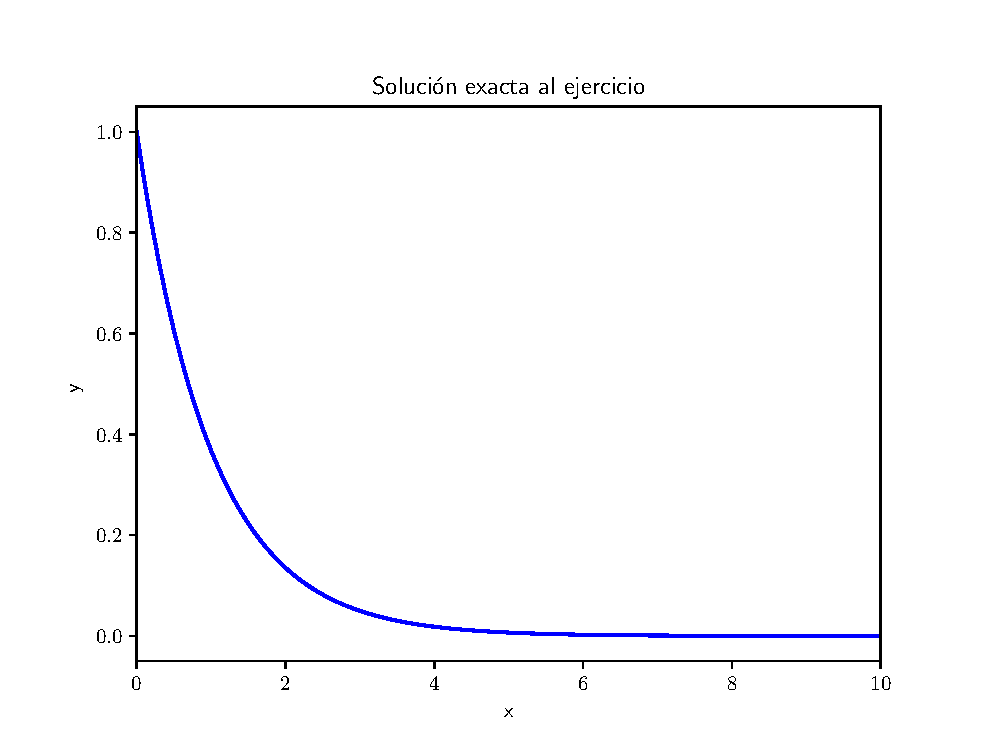
\includegraphics[scale=0.55]{Imagenes/plot_rk4_ejercicio_02_02.eps}
\end{figure}
\end{frame}
\begin{frame}
\frametitle{Código para resolver el ejercicio}
En el código utilizamos la función \funcionazul{integraorden4}.
\\
\bigskip
\pause
\textbf{Ejercicio a cuenta: } incluye una rutina de graficación para obtener la solución numérica y la exacta. Envía las dos gráficas por correo.
\end{frame}
\begin{frame}[allowframebreaks, fragile]
\frametitle{Código para resolver el ejercicio 2}
\begin{lstlisting}[caption=Código con el método RK4 que resuelve el ejercicio]
from metodosDirectos import integraorden4
import numpy as np

def f(x, y):
	f = np.zeros(1)
	f[0] = 3 * y[0] - 4 * np.exp(-x)
	return f

x = 0.0
xAlto = 10.0
y = np.array([1.])
h = 0.1

X, Y = integraorden4(f, x, y, xAlto, h)
s_Exacta = np.exp(-X)
\end{lstlisting}
\end{frame}
\begin{frame}
\frametitle{Gráfica de la solución numérica}
\begin{figure}
	\centering
	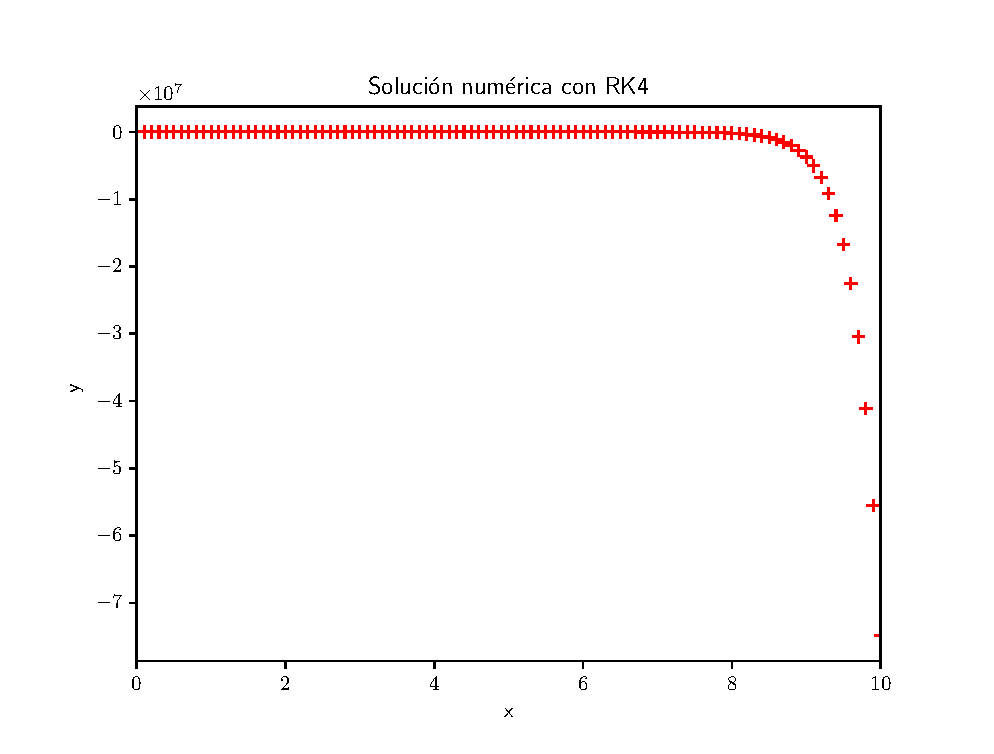
\includegraphics[scale=0.545]{Imagenes/plot_rk4_ejercicio_02_01.eps}
\end{figure}
\end{frame}
\begin{frame}
\frametitle{¿Qué ha pasado?}
Está claro que algo salió mal!!.
\\
\bigskip
\pause
De acuerdo con la solución analítica, $y$ debería aproximarse a cero al aumentar $x$, \pause pero el resultado muestra la tendencia opuesta: después de una disminución inicial, la magnitud de $y$ aumenta drásticamente.
\end{frame}
\begin{frame}
\frametitle{¿Qué salió mal?}
La explicación se encuentra observando más de cerca la solución analítica.
\\
\bigskip
\pause
La solución general de la ecuación diferencial dada es:
\pause
\begin{align*}
y = C \, e^{3 x} + e^{-x}
\end{align*}
que se puede verificar por sustitución.
\end{frame}
\begin{frame}
\frametitle{Revisando la solución analítica}
Con la condición inicial $y (0) = 1$, \pause se tiene que: $C = 0$, \pause por lo que la solución al problema, es la esperada: $y = e^{-x}$
\end{frame}
\begin{frame}
\frametitle{Causa del problema}
La causa del problema en la solución numérica es el término latente $C \, e^{3 x}$.
\\
\bigskip
\pause
Supongamos que la condición inicial contiene un pequeño error $\varepsilon$, por lo que tenemos $y (0) = 1 + \varepsilon$. \pause Esto cambia la solución analítica a:
\pause
\begin{align*}
y = \varepsilon \, e^{3 x} + e^{-x}
\end{align*}
\end{frame}
\begin{frame}
\frametitle{Término dominante}
Ahora vemos que el término que contiene el error $\varepsilon$ se vuelve dominante a medida que $x$ aumenta.
\\
\bigskip
\pause
Debido a que los errores inherentes a la solución numérica tienen el mismo efecto que pequeños cambios en las condiciones iniciales.
\end{frame}
\begin{frame}
\frametitle{Hecho muy importante}
Concluimos que nuestra solución numérica es víctima de \textcolor{red}{inestabilidad numérica} debido a la sensibilidad de la solución a las condiciones iniciales.
\\
\bigskip
\pause
\textbf{\textcolor{airforceblue}{Moraleja: }} No hay que confiar ciegamente en los resultados de la integración numérica.
\end{frame}
\begin{frame}
\frametitle{Ejercicios a cuenta}
\setbeamercolor{item projected}{bg=red,fg=white}
\setbeamertemplate{enumerate items}{%
\usebeamercolor[bg]{item projected}%
\raisebox{1.5pt}{\colorbox{bg}{\color{fg}\footnotesize\insertenumlabel}}%
}
\begin{enumerate}
\item La posición de equilibrio de un cilindro flotante es $h = r$. Si el cilindro se desplaza a la posición $h = 1.5 \: r$ y se libera, la ecuación diferencial que describe el movimiento es
\begin{align*}
\ddot{y} = \dfrac{2}{\pi} \: \left[ \tan^{-1} \: \dfrac{1 - y}{\sqrt{2 \: y - y^{2}}} + (1 - y) \: \sqrt{2 \: y - y^{2}} \right]
\end{align*}
donde $y = h / r$.
\seti 
\end{enumerate}
\end{frame}

\subsection*{Ejercicios a cuenta}

\begin{frame}
\frametitle{Ejercicios a cuenta}
\begin{figure}[H]
\centering
\begin{tikzpicture}
	\node[circle, draw, minimum size=4cm] (A) at  (0,0) {};
	\draw [dash pattern={on 7pt off 2pt on 1pt off 3pt}] (-2.5, 0) -- (2.5, 0);
	\draw [dash pattern={on 7pt off 2pt on 1pt off 3pt}] (0, -2.5) -- (0, 2.5);
	\draw [arrows=->, thick] (0,0) -- ++(45:2) node [midway, above] {$r$};
	\draw (0, -2) -- (3.5, -2);
	\draw [arrows=->, thick, color=white] (0,0) -- ++(210:2) coordinate (B);
	\draw [arrows=->, thick, color=white] (0,0) -- ++(-30:2) coordinate (C);
	\draw (-4, -1) -- (B);
	\draw [dash pattern=on 3pt off 2pt] (B) -- (C);
	\draw (C) -- (3.5, -1);
	\draw [arrows=<->] (3.2, -1) -- (3.2, -2) node [midway, left] {$h$};
	\draw (-4, 0.25) node {Nivel del agua};
	\draw [arrows=->] (-3.7, 0.1	) -- (-3.5, -1);
\end{tikzpicture}
\end{figure}
\end{frame}
\begin{frame}
\frametitle{Ejercicios a cuenta}
Grafica $h/r$ desde $t = 0$ hasta $t = 6$. A partir de la gráfica estima el período del movimiento resultante.
\end{frame}
\begin{frame}
\frametitle{Ejercicios a cuenta}
\setbeamertemplate{enumerate items}{%
\usebeamercolor[bg]{item projected}%
\raisebox{1.5pt}{\colorbox{bg}{\color{fg}\footnotesize\insertenumlabel}}%
}
\begin{enumerate}
\conti
\item Un paracaidista de masa $m$ en una caída libre vertical experimenta una fuerza aerodinámica de arrastre $F_{\text{D}} = C_{D} \, \dot{y}^{\, 2}$, donde $y$ se mide hacia abajo desde el comienzo de la caída. La ecuación diferencial que describe la caída es:
\begin{align*}
\ddot{y} = g - \dfrac{C_{\text{D}}}{m} \, \dot{y}^{\, 2}
\end{align*}
\end{enumerate}
\end{frame}
\begin{frame}
\frametitle{Ejercicios a cuenta}
Calcula el tiempo de caída desde una altura de $\SI{5000}{\meter}$. Usa los valores de $g = \SI{9.81}{\meter\per\square\second}$, $C_{\text{D}} = \SI{0.2028 }{\kilo\gram\per\metre}$ y $m = \SI{80}{\kilo\gram}$.
\end{frame}

\section{Estabilidad y rigidez}
\frame{\tableofcontents[currentsection, hideothersubsections]}
\subsection{Definiciones}

\begin{frame}
\frametitle{Concepto de estabilidad}
Hablando de manera general, un método de integración se dice que \textcolor{blue}{es estable} si los efectos de errores locales, no se acumulan progresivamente, es decir, si el error global permanece acotado.
\end{frame}
\begin{frame}
\frametitle{Concepto de estabilidad}
Si el método \textcolor{red}{es inestable}, si el error global se incrementa de manera exponencial, generando eventualmente un desbordamiento (overflow).
\\
\bigskip
\pause
La estabilidad no tiene nada que ver con la precisión, de hecho, un método impreciso puede ser muy estable.
\end{frame}
\begin{frame}
\frametitle{Determinantes de la estabilidad}
La estabilidad está determinada por tres factores:
\pause
\setbeamercolor{item projected}{bg=ao,fg=beige}
\setbeamertemplate{enumerate items}{%
\usebeamercolor[bg]{item projected}%
\raisebox{1.5pt}{\colorbox{bg}{\color{fg}\footnotesize\insertenumlabel}}%
}
\begin{enumerate}[<+->]
\item Las ecuaciones diferenciales.
\item El método de solución.
\item El valor del incremento $h$.
\end{enumerate}
\pause
Desafortunadamente, no es fácil determinar de antemano la estabilidad, a menos que la ecuación diferencial sea lineal.
\end{frame}

\subsection{Estabilidad del método de Euler}

\begin{frame}
\frametitle{Estabilidad del método de Euler}
Con el fin de ilustar la estabilidad, consideremos el problema lineal:
\pause
\begin{align*}
\pderivada{y} = - \lambda \, y \hspace{2cm} y (0) = \beta
\end{align*}
donde $\lambda$ es una constante positiva.
\\
\medskip
\pause
La solución exacta de este problema es:
\pause
\begin{align*}
y (x) = \beta \, e^{- \lambda x}
\end{align*}
\end{frame}
\begin{frame}
\frametitle{Solución numérica}
Veamos qué pasa cuando intentamos resolver numéricamente esta ecuación con el método de Euler:
\pause
\begin{align*}
y (x + h) = y (x) + h \, \pderivada{y} (x)
\end{align*}
\pause
sustituimos $\pderivada{y} (x) = - \lambda \, y (x)$, para obtener:
\pause
\begin{align*}
y (x + h) = (1 - \lambda \, h) \, y (x)
\end{align*}
\end{frame}
\begin{frame}
\frametitle{Regiones de estabilidad}
\begin{align*}
y (x + h) = (1 - \lambda \, h) \, y (x)
\end{align*}
Si $\abs{1 - \lambda \, h} > 1$, se nota claramente que \textcolor{red}{el método es inestable}, \pause ya que el valor de $\abs{y}$ se incrementa en cada paso de integración.
\\
\medskip
\pause
Por tanto, \pause \textcolor{blue}{el método de Euler es estable} solamente si $\abs{1 - \lambda \, h} \leq 1$, o
\begin{align*}
h \leq \dfrac{2}{\lambda}
\end{align*}
\end{frame}
\begin{frame}
\frametitle{Extendiendo los resultados}
Los resultados se pueden extender a un sistema de $n$ ecuaciones diferenciales de la forma:
\pause
\begin{align*}
\mathbf{\pderivada{y}} = - \mathbf{\Lambda \, y}
\end{align*}
donde $\mathbf{\Lambda}$ es una matriz constante con eigenvalores positivos $\lambda_{i}$, con $i = 1, 2, \ldots, n$.
\end{frame}
\begin{frame}
\frametitle{Extendiendo los resultados}
Se puede demostrar que el método de integración de Euler es estable si:
\pause
\begin{align*}
h < \dfrac{2}{\lambda_{\text{max}}}
\end{align*}
donde $\lambda_{\text{max}}$ es el valor propio mayor de $\mathbf{\Lambda}$.
\end{frame}

\section{Rigidez}
\frame{\tableofcontents[currentsection, hideothersubsections]}
\subsection{Definición}

\begin{frame}
\frametitle{El concepto de rigidez}
Un problema de valores iniciales se dice que es \textbf{\emph{\textcolor{carmine}{rígido}}}, si algunos de los elementos del vector solución $\mathbf{y} (x)$ varían mucho más rápido con respecto a $x$, que otros.
\end{frame}
\begin{frame}
\frametitle{El concepto de rigidez}
La rigidez puede predecirse fácilmente del conjunto de ED $\mathbf{\pderivada{y}} = - \mathbf{\Lambda \, y}$ con una matriz de coeficientes constantes $\mathbf{\Lambda}$.
\end{frame}
\begin{frame}
\frametitle{Solución al sistema}
La solución de esas ecuaciones es:
\pause
\begin{align*}
\mathbf{y} (x) = \nsum_{i} C_{i} \, \mathbf{v}_{i} \, \exp(-\lambda_{i} \, x)
\end{align*}
donde $\lambda_{i}$ son los eigenvalores de $\mathbf{\Lambda}$ y $\mathbf{v}_{i}$ son los correspondientes eigenvectores.
\end{frame}
\begin{frame}
\frametitle{Rigidez del problema}
Es evidente que el problema es rígido si hay una gran disparidad en las magnitudes de los eigenvalores positivos.
\end{frame}
\begin{frame}
\frametitle{Integración de problemas rídigos}
La integración numérica de las ecuaciones rígidas requiere un cuidado especial.
\\
\bigskip
\pause
El tamaño del paso $h$ necesario para la estabilidad está determinado por el valor propio más grande ($\lambda_{max}$), \pause aunque si los términos $\exp(-\lambda_{max} \, x)$ en la solución decaen muy rápidamente y se vuelven insignificantes a medida que nos alejamos del origen.
\end{frame}
\begin{frame}
\frametitle{Ejemplo de un problema rígido}
Por ejemplo, sea la siguiente EDO:
\begin{align*}
\sderivada{y} + 1001 \, \pderivada{y} + 1000 \, y = 0
\end{align*}
\pause
usando $y_{0} = y$ junto con $y_{1} = y_{1}$, el conjunto equivalente de EDO1, resulta ser:
\pause
\begin{align*}
\pderivada{\mathbf{y}} = \begin{bmatrix}
y_{1} \\
-1000 \, y_{0} - 1001 \, y_{1}
\end{bmatrix}
\end{align*}
\end{frame}
\begin{frame}
\frametitle{Ejemplo de un problema rígido}
En este caso:
\pause
\begin{align*}
\mathbf{\Lambda} = \begin{bmatrix}
0 & -1 \\
1000 & 1001 
\end{bmatrix}
\end{align*}
\end{frame}
\begin{frame}
\frametitle{Eigenvalores}
Los eigenvalores son las raíces de:
\pause
\begin{align*}
\abs{\mathbf{\Lambda} - \lambda \, \mathbf{I}} = \begin{vmatrix}
- \lambda & -1 \\
1000 & 1001 - \lambda
 \end{vmatrix} = 0
\end{align*}
\pause
expandiendo el determinante, tenemos que:
\pause
\begin{align*}
- \lambda (1001 - \lambda) + 1000 = 0
\end{align*}
\pause
las soluciones son $\lambda_{1} = 1$ y $\lambda_{2} = 1000$.
\end{frame}
\begin{frame}
\frametitle{Problema rígido}
Claramente la ecuación es rígida; se necesita que $h < 2/\lambda_{2} = 0.002$ para que el método de Euler sea estable.
\\
\medskip
\pause
El método de Runge-Kutta tendría aproximadamente la misma limitación en el tamaño del paso.
\end{frame}

\section{Método Predictor-Corrector Euler}
\frame{\tableofcontents[currentsection, hideothersubsections]}
\subsection{Construyendo el método}

\begin{frame}
\frametitle{Mejora en el método de Euler}
Una forma práctica de superar la baja precisión del método de Euler es elevar el orden de la aproximación aplicando su variante llamada  \textoazul{método predictor - corrector} de Euler, que opera con dos estimaciones de solución en cada paso de propagación.
\end{frame}
\begin{frame}
\frametitle{Método predictor - corrector}
\begin{align}
\overline{y}_{m + 1} &= y_{m} + h \: f (t_{m}, y_{m}), \hspace{0.3cm} m = 1, 2, 3, \ldots \label{eq:ecuacion_12_17} \\
y_{m + 1} &= y_{m} + \dfrac{h}{2} \: [ f(t_{m}, y_{m}) + f (t_{m} + h, \overline{y}_{m + 1})] \label{eq:ecuacion_12_18}
\end{align}
\pause
donde:
\setbeamercolor{item projected}{bg=bananayellow,fg=bleudefrance}
\setbeamertemplate{enumerate items}{%
\usebeamercolor[bg]{item projected}%
\raisebox{1.5pt}{\colorbox{bg}{\color{fg}\footnotesize\insertenumlabel}}%
}
\begin{enumerate}[<+->]
\item $\overline{y}_{m + 1}$ es el valor predictor.
\item $y_{m + 1}$ es el valor corregido.
\end{enumerate}
\end{frame}
\begin{frame}
\frametitle{Valor predictor}
El valor predictor de la solución $ \overline{y}_{m + 1}$ se obtiene del método de Euler, de la expresión predictora (ec. \ref{eq:ecuacion_12_17}).
\\
\bigskip
\pause
Se utiliza para estimar la propagación de la derivada $f (t_{m} + h, \overline{y}_{m + 1})$
\end{frame}
\begin{frame}
\frametitle{Valor corregido}
El valor de la solución corregida $y_{m + 1}$ se obtiene de la fórmula de corrección (ec. \ref{eq:ecuacion_12_18}), que utiliza el promedio de la derivada estimada en el intervalo $[x_{m}, x_{m + 1}]$:
\pause
\begin{align*}
\dfrac{\big[ f (t_{m}, y_{m}) + f (t_{m} + h, \overline{y}_{m + 1}) \big]}{2}
\end{align*}
\end{frame}
% \begin{frame}
% \frametitle{Casos especiales de Runge-Kutta}
% Veremos más adelante que los métodos de Euler básicos y el predictor - corrector son casos particulares de una familia completa de algoritmos, conocidos como \textoazul{métodos de Runge-Kutta}.
% \end{frame}
\begin{frame}
\frametitle{Compración con el RK2}
% El método básico de Euler es equivalente al método de primer orden de Runge-Kutta (RK1).
% \\
% \bigskip
El algoritmo predictor - corrector de Euler es de orden $\order{h^2}$, es equivalente al método de Runge-Kutta de segundo orden (RK2). 
\end{frame}
\begin{frame}
\frametitle{Mayor precisión del método}
La precisión superior del algoritmo predictor-corrector Euler obviamente se produce a expensas de un doble número de evaluaciones de las funciones del lado derecho $f (x, y)$ de las EDO.
\end{frame}

\subsection{Ejercicio 1}

\begin{frame}
\frametitle{Estabilidad y precisión del método predictor-corrector}
Para revisar la precisión y estabilidad de el método predictor-corrector de Euler, regresemos al siguiente problema:
\pause
\begin{align}
\sderivada{y} + y &= 0 \label{eq:ecuacion_12_19} \\
y(0) &=  y_{0}, \hspace{0.3cm} \pderivada{y} (0) = \pderivada{y}_{0} \label{ec:ecuacion_12_20}
\end{align}
\end{frame}
\begin{frame}
\frametitle{Solución exacta}
Ya habíamos determinado que el problema con los valores iniciales dados:
\pause
\begin{align*}
y_{1} (0) = 0 \hspace{0.3cm} y_{2} (0) = 1
\end{align*}
tiene como solución exacta:
\pause
\begin{align*}
y_{1} (t) = \sin t, \hspace{0.3cm} y_{2} (t) = \cos t
\end{align*}
\end{frame}
\begin{frame}
\frametitle{Solución y gráficas del problema}
En la presentación anterior del Tema, se resolvió el problema con el método de Euler.
\pause
Obteniendo las siguientes gráficas:
\end{frame}
\begin{frame}
\frametitle{Solución periódica}
\begin{figure}
    \centering
    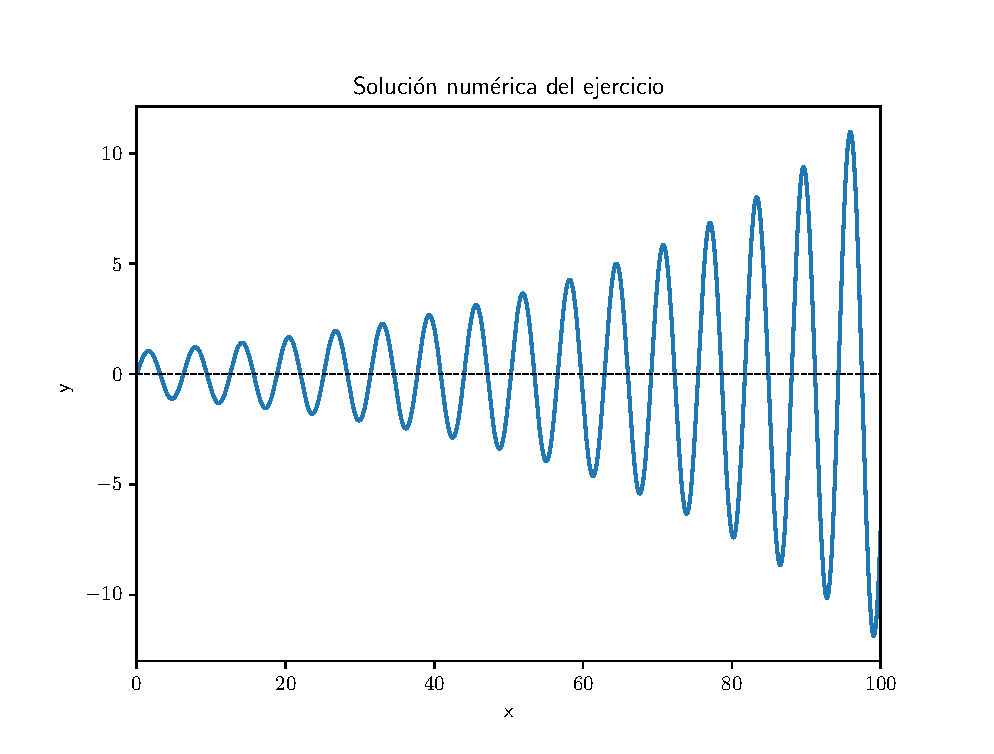
\includegraphics[scale=0.55]{Imagenes/plot_euler_ejercicio_04.eps}
\end{figure}
\end{frame}
\begin{frame}
\frametitle{¿Qué está ocurriendo?}
Sabemos que la solución de la EDO2 es periódica, no hay factores de amortiguamiento ni otro elemento que modifique la amplitud de la solución.
\\
\bigskip
\pause
Pero vemos en la gráfica que aumenta la amplitud conforme transcurre el tiempo.
\end{frame}
\begin{frame}
\frametitle{Diagrama espacio - fase}
Otra manera con la que se revisó si hay una inconsistencia en los resultados, fu la de graficar el espacio fase.
\end{frame}
\begin{frame}
\frametitle{¿Cómo debe de ser?}
El estado fase de la EDO2 supone que no hay pérdida de energía, por lo que tendríamos una gráfica cerrada y de trazo uniforme.
\end{frame}
\begin{frame}
\frametitle{Gráfica del espacio fase}
\begin{figure}
	\centering
	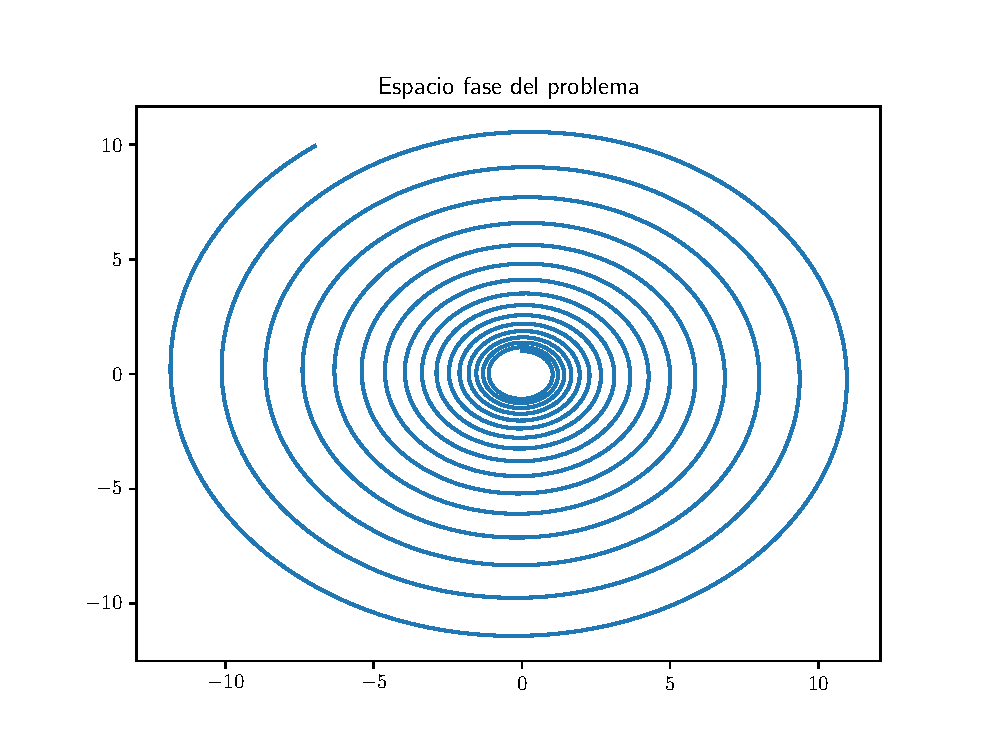
\includegraphics[scale=0.55]{Imagenes/plot_euler_ejercicio_05.eps}
\end{figure}
\end{frame}
\begin{frame}
\frametitle{Resultado}
El estado fase presenta una trayectoria abierta, por lo que no hay correspondencia con el fenómeno.
\\
\bigskip
\pause
El método de Euler no funciona del todo bien con la EDO2 del tipo estudiado.
\end{frame}
\begin{frame}
\frametitle{Usando el predictor - corrector}
Ahora usaremos el algoritmo de Euler predictor - corrector para resolver el ejercicio y contrastar los resultados.
\\
\bigskip
\pause
Conviene tener la siguiente función dentro del módulo \funcionazul{metodosDirectos}.
\end{frame}
\begin{frame}[allowframebreaks, fragile]
\frametitle{Método predictor - corrector de Euler}
\begin{lstlisting}[caption=Método predictor - corrector de Euler]
def eulerPC(t, ht, y, n, Func):

    f1 = [0] * (n); f2 = [0] * (n)
    yt = [0] * (n)
 
    # Lado derecho de la EDO en t
    Func(t, y, f1)

    # Paso predictor
    for i in range(n): yt[i] = y[i] + ht * f1[i]
    
    # Lado derecho de la EDO en t+ht
    Func(t + ht, yt, f2)
 
    ht2 = ht/2e0

    # Paso corrector
    for i in range(n): y[i] += ht2 * (f1[i] + f2[i])
    
    return y
\end{lstlisting}
\end{frame}
\begin{frame}
\frametitle{Código completo para la solución}
El siguiente código es la implementación del método predictor-corrector de Euler.
\\
\bigskip
\pause
Toma en cuenta que falta incluir la rutina de graficación para obtener la gráfica de la solución de la EDO y la gráfica el espacio fase.
\end{frame}
\begin{frame}[allowframebreaks, fragile]
\frametitle{Código completo para la solución}
\begin{lstlisting}[caption=Código completo con el método predictor-corrector de Euler]
from metodosDirectos import eulerPC
import numpy as np

def f(x, y, f):
    f[0] = y[1]
    f[1] = -y[0]
    return f

n = 2
x = 0.0
xAlto = 100.0
y = np.array([0., 1.])
h = 0.05

nt = int(xAlto/h + 0.5) + 1

y1 = np.zeros(nt+1)
y2 = np.zeros(nt+1)

y1[0] = y[0]
y2[0] = y[1]
it = 1

while (x + h <= xAlto):
    eulerPC(x, h, y, n, f)
    x += h
    it += 1
    y1[it] = y[0]
    y2[it] = y[1]
\end{lstlisting}
\end{frame}
\begin{frame}
\frametitle{Las gráficas obtenidas}
A continuación se presentan las gráficas tanto de la solución de la EDO, como la gráfica del espacio fase.
\end{frame}
\begin{frame}
\frametitle{Solución de la EDO con eulerPC}
\begin{figure}
	\centering
	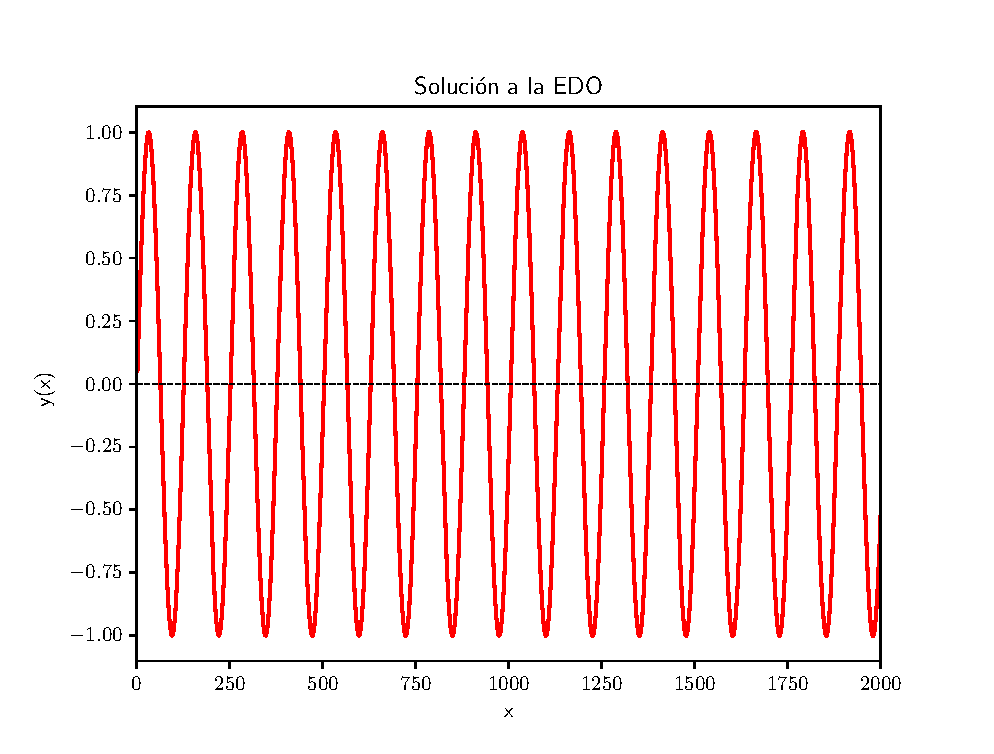
\includegraphics[scale=0.55]{Imagenes/plot_eulerPC_ejercicio_01.eps}
\end{figure}
\end{frame}
\begin{frame}
\frametitle{Espacio fase de la EDO con eulerPC}
\begin{figure}
	\centering
	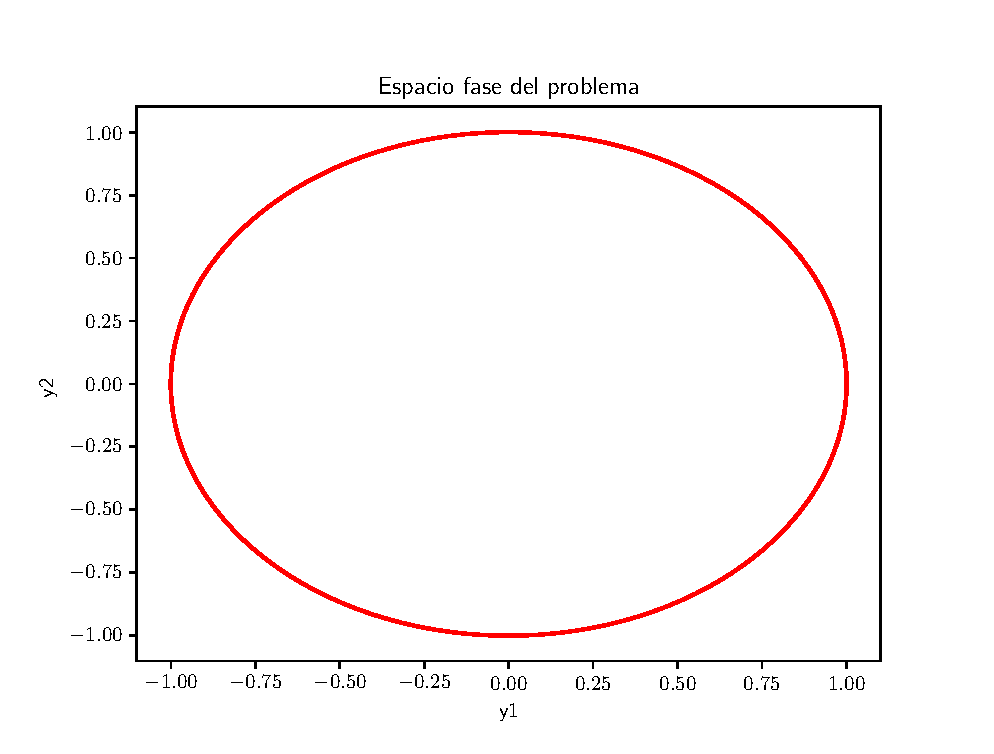
\includegraphics[scale=0.55]{Imagenes/plot_eulerPC_ejercicio_02.eps}
\end{figure}
\end{frame}
\begin{frame}
\frametitle{Conclusión}
Vemos que el método de Euler predictor - corrector, corrige la falla en la estabilidad de la solución.
\end{frame}

\end{document}